% -*- mode: latex -*-
\documentclass[landscape]{slides}
\usepackage{times}

\usepackage{alltt,sped,epsfig,colordvi}
\frenchspacing

\addtolength\topmargin{-.4in}
\addtolength\textheight{.5in}

\def\bullet{\char"D5\relax}
\def\textbullet{\char"D5\relax}
\def\...{\,.\,.\,.\,\ignorespaces}%

\newcommand{\edots}{\unskip\penalty10$\,$\dots\penalty10\relax}%

\def\BTWO#1#2{\noindent%
\begin{tabular}{@{}p{#1}p{#2}@{}}\afterbulletfalse\vfil}
\def\XTWO{\vskip-\lastskip\vfil&\afterbulletfalse}
\def\ETWO{\end{tabular}\par}

\def\sbseries{\fontseries{s}\selectfont}

\catcode`\>\active\catcode`\_\active
\newenvironment{clicklang}
{\begin{ttfamily}
\begin{small}
\parskip=0pt
\obeylines\obeyspaces\catcode`\>\active\def>{\char`\>{}}\catcode`\_\active\def_{\char`\_}%
\def\backslash{\char`\\}%
\def\{{\char`\{}\def\}{\char`\}}}{\end{small}\end{ttfamily}}
\newenvironment{clicklangsm}
{\begin{ttfamily}
\begin{tiny}
\parskip=0pt
\obeylines\obeyspaces\catcode`\>\active\def>{\char`\>{}}\catcode`\_\active\def_{\char`\_}%
\def\backslash{\char`\\}%
\def\{{\char`\{}\def\}{\char`\}}}{\end{tiny}\end{ttfamily}}
\catcode`\>=12\catcode`\_=8%

\newif\ifafterbullet
%\def\ORN{{\usefont{OT1}{Minion}{m}{orn}\MidnightBlue{v}}}%
\def\ORNA{{\LARGE\usefont{OT1}{CaravanLH}{m}{orn3}\MidnightBlue{*}}}%
\def\ORN{{\large\usefont{OT1}{CaravanLH}{m}{orn3}\Goldenrod{\%}}}%
\def\T#1{\begin{center}\large\bfseries{\PineGreen{#1}}\par\vskip-40pt\ORN\end{center}%
  \vskip30pt\afterbulletfalse\parskip0pt}
\def\TT#1{\begin{center}\large\bfseries{\PineGreen{#1}}\end{center}%
  \vskip30pt\afterbulletfalse\parskip0pt}
\def\S{\afterbullettrue}
\def\B{\sbseries\doedbullet{20pt}{\bullet~~}}
\def\NB#1{\doedbullet{20pt}{#1.~~}\ignorespaces}
\def\BB{\mdseries\doedbullet{6pt}{\hskip0.6in\relax}}
\def\BBB{\mdseries\doedbullet{6pt}{\hskip1in\relax}}
\def\doedbullet#1#2{\ifafterbullet\par\vskip-\lastskip\vskip#1\fi
  \setbox0\hbox{#2}\hangafter1\hangindent\wd0\noindent\box0
  \raggedright\afterbullettrue}

\makeatletter
\def\makeslidenum#1{\Gray{\fontseries{u}\selectfont#1}}%
\def\ps@slide{%
 \def\@oddfoot{\@mainsize \mbox{}\hfil\lower0.3in\hbox{\makeslidenum{\theslide}}\hfil\mbox{}}%
 \def\@oddhead{}%
 \def\@evenfoot{\@mainsize \mbox{}\hfil\lower0.3in\hbox{\makeslidenum{\theslide}}\hfil\mbox{}}%
 \def\@evenhead{}}
\def\ps@overlay{%
 \def\@oddfoot{\@mainsize \mbox{}\hfil\lower0.3in\hbox{\makeslidenum{\theslide}}\hfil\mbox{}}%
 \def\@oddhead{}%
 \def\@evenfoot{\@mainsize \mbox{}\hfil\lower0.3in\hbox{\makeslidenum{\theslide}}\hfil\mbox{}}%
 \def\@evenhead{}}

\def\cppfont{\ttfamily\fontsize{21}{21}\selectfont}

\begin{document}
\rmfamily
\renewcommand{\theslide}{\arabic{slide}}


\begin{slide}
\begin{center}
{\LARGE \Red{\sbseries{XORP: An eXtensible Open Router Platform}}} \\
\vskip20pt

\ORNA

\vskip5pt
\begin{tabular}{c}
Atanu Ghosh \qquad Mark Handley \qquad Orion Hodson \\
\textbf{Eddie Kohler} \qquad Pavlin Radoslavov \\
\Gray{International Computer Science Institute}
\end{tabular}

\vskip-5pt
\begin{tabular}{c@{\qquad\qquad}c}
Adam Greenhalgh & Luigi Rizzo \\
\Gray{University College London} & \Gray{University of Pisa}
\end{tabular}
\end{center}
\end{slide}


\begin{slide}
\T{Networking research: divorced from reality?}

\B Gap between research and practice in routing and forwarding
\B Most of the important Internet protocols originated in research, often
at universities.
\BB It used to be that researchers designed systems, \emph{built
implementations}, \emph{tried them out}, and standardized the ones that
\emph{survived and proved useful}.
\BB What happened?
\end{slide}


\begin{slide}
\T{Networking research: why the divorce?}

\B The commercial Internet
\BB Network stability is critical, so experimentation is difficult
\BB Major infrastructure vendors not motivated to support experimentation
\B Network simulators
\BB High-quality simulators make a lingua franca for research
\end{slide}


\begin{slide}
\T{Simulation is not a substitute for experimentation}

\B Many questions require real-world traffic and/or routing information 
\B Most grad students:
\BB Give up, implement their protocol in \emph{ns}
\BB Set \emph{ns} parameters based on guesses, existing scripts
\BB Write a paper that may or may not bear any relationship to reality
\B We need to be able to run experiments when required!
\end{slide}


\begin{slide}
\T{The state of the art}

\B Open APIs facilitate end-system protocol development
\BB WWW, RTP, SIP, RTSP, \dots
\B Open-source OSes do the same for kernel changes
\BB TCP SACK, IGMPv3, \dots
\BB Also a history of experimentation in commercial OSes (affiliated labs)
\B Overlay networks may help with end-system/network interactions
\BB Field in its infancy
\end{slide}


\begin{slide}
\T{What about protocols that affect the routers?}

\B Option 1:
\BB Persuade Cisco to implement your protocol;
\BB Persuade ISPs that your protocol won't destabilize their networks;
\BB Conduct experiment.
\B Option 2:
\BB Implement routing protocol part in MRTd, GateD, or Zebra;
\BB Implement forwarding part in FreeBSD, Linux, Click, Scout, \dots;
\BB Persuade network operators to replace their Ciscos with your PC;
\BB Conduct experiment.
\end{slide}


\begin{slide}
\T{Likelihood of success?}

\centering
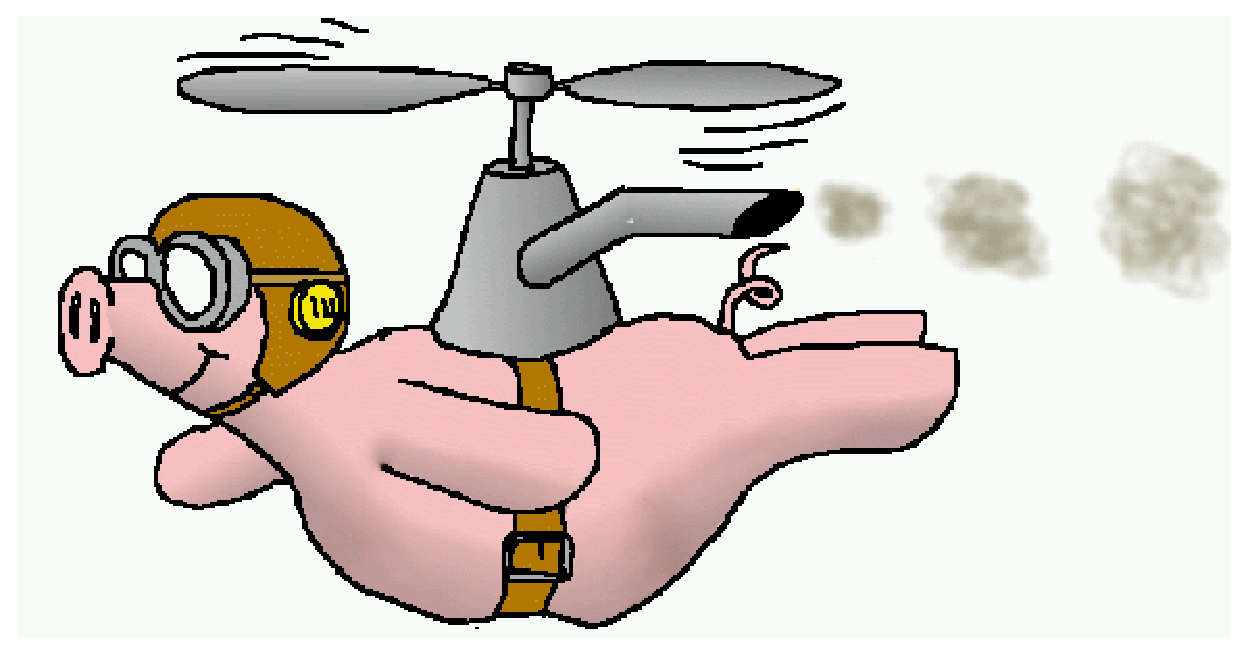
\epsfig{file=flyingpig.eps,width=.8\hsize}
\end{slide}


\begin{slide}
\T{Possible solutions}

\B Solution 1:
\BB A router vendor opens their development environment and APIs.
\BB Thus, new router applications can be written and deployed by third
parties.
\BB Basic router functionality cannot be changed.
\B Solution 2:
\BB Someone (\emph{hint, hint}) builds a complete open-source router
software stack explicit designed for extensibility \emph{and} robustness.
\BB Adventurous network operators deploy this router on their
networks;
it develops a reputation for stability and configurability.
\BB Result: a fully extensible platform suitable for research \emph{and}
deployment.
\end{slide}


\begin{slide}
\T{XORP}

\B eXtensible Open Router Platform
\B Complete software stack for an IP router, including routing protocols,
management interfaces, and forwarding path
\end{slide}


\begin{slide}
\enlargethispage{3\baselineskip}
\TT{Architecture}

\begin{center}
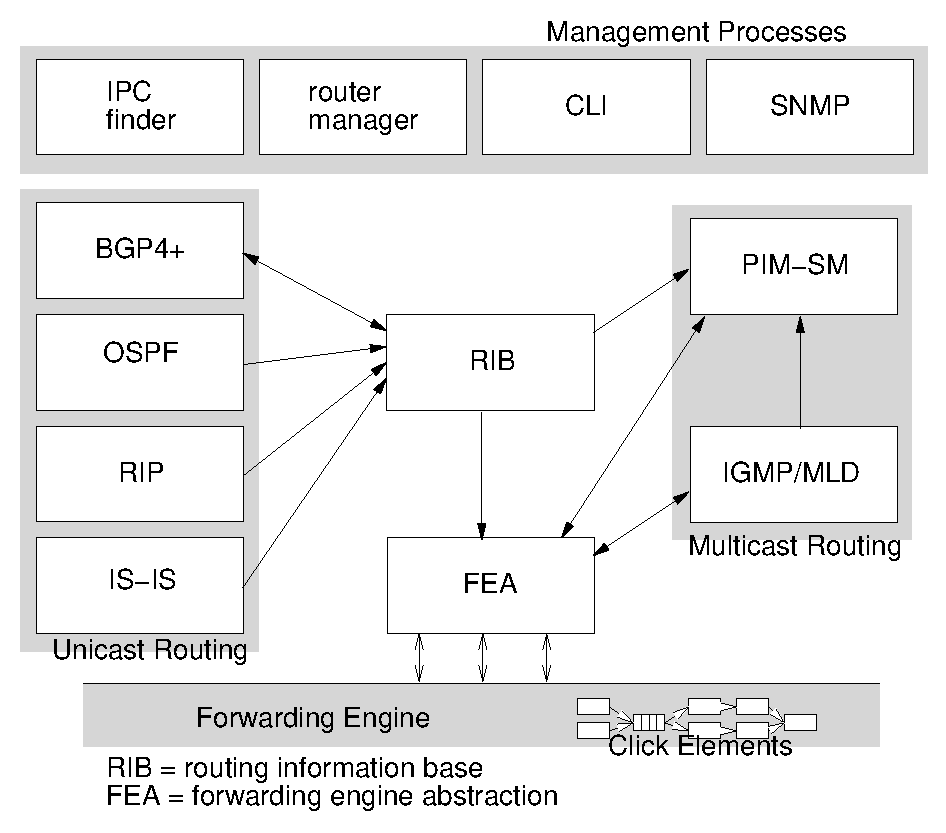
\epsfig{file=processes3.ps,width=.7\hsize}
\end{center}
\end{slide}


\begin{slide}
\T{Four challenges}

\B Features
\BB Real-world routers must support a long feature list
\B Extensibility
\BB Every aspect of the router should be extensible
\BB Multiple extensions should be able to coexist
\B Performance
\BB Not core routers, but edge routing is hard enough
\BB Raw forwarding performance, scalability in routing table size
\B Robustness
\BB Must not crash or misroute packets
\end{slide}


\let\Future\Tan
\begin{slide}
\T{Features}

\B IPv4 and \Future{IPv6}
\B Unicast routing protocols
\BB BGP4+, OSPF, RIPv2/RIPng, \Future{Integrated IS-IS}
\B Multicast
\BB PIM-SM/SSM, IGMPv3/MLD
\B \Future{DHCP, PPP}
\B Management
\BB \Future{SNMP,} command line, \Future{WWW}
\B Forwarding elements
\BB Route lookup, filter/firewall, ARP, AQM, \Future{encapsulation}
\end{slide}


\begin{slide}
\T{Extensibility: Intra-router APIs}

\B Separate abstract request (API) from concrete request (which process?
which arguments? which version?)
\B In particular, the caller:
\BB Should not care about IPC mechanism
\BB Should not know in advance which process is relevant
\BB \dots unless required
\end{slide}


\begin{slide}
\T{Extensibility: XORP Resource Locators}

\B XORP IPC mechanism
\BB Like URLs for IPC
\begin{center}
\texttt{finder://fea/fea/1.0/add\char`\_address4?vif:txt=fxp0\&addr:ipv4=10.0.0.1}
\vskip20pt
\end{center}
\textWhite
\B Library marshals arguments, implements transport, handles responses
\B Redirection into a single XRL or an XRL sequence
\B Programmer explicitly handles failure
\textBlack
\end{slide}


\def\LN#1{\setbox0\hbox{\lower\baselineskip\hbox{\rmfamily\BrickRed{#1}}}\wd0=0pt\ht0=0pt\dp0=0pt\box0\relax}
\def\RN#1{\setbox0\hbox{\lower\baselineskip\hbox to0pt{\hskip0pt plus-1000pt \rmfamily\BrickRed{#1}}}\ht0=0pt\dp0=0pt\box0\relax}
\let\t\texttt

\begin{overlay}
\T{Extensibility: XORP Resource Locators}

\B XORP IPC mechanism
\BB Like URLs for IPC
\begin{center}
\texttt{\LN{IPC mechanism: \t{finder}, \t{xudp}, \t{snmp}, \dots}\Red{finder}://fea/fea/1.0/add\char`\_address4?vif:txt=fxp0\&addr:ipv4=10.0.0.1}
\vskip20pt
\end{center}
\textWhite
\B Library marshals arguments, implements transport, handles responses
\B Redirection into a single XRL or an XRL sequence
\B Programmer explicitly handles failure
\textBlack
\end{overlay}

\begin{overlay}
\T{Extensibility: XORP Resource Locators}

\B XORP IPC mechanism
\BB Like URLs for IPC
\begin{center}
\texttt{finder://\LN{Module/process name: \t{fea}, \t{rib}, \t{bgp}, \dots}\Red{fea}/fea/1.0/add\char`\_address4?vif:txt=fxp0\&addr:ipv4=10.0.0.1}
\vskip20pt
\end{center}
\textWhite
\B Library marshals arguments, implements transport, handles responses
\B Redirection into a single XRL or an XRL sequence
\B Programmer explicitly handles failure
\textBlack
\end{overlay}

\begin{overlay}
\T{Extensibility: XORP Resource Locators}

\B XORP IPC mechanism
\BB Like URLs for IPC
\begin{center}
\texttt{finder://fea/\LN{Interface name: \t{fea}, \t{routing-process}, \dots}\Red{fea}/1.0/add\char`\_address4?vif:txt=fxp0\&addr:ipv4=10.0.0.1}
\vskip20pt
\end{center}
\textWhite
\B Library marshals arguments, implements transport, handles responses
\B Redirection into a single XRL or an XRL sequence
\B Programmer explicitly handles failure
\textBlack
\end{overlay}

\begin{overlay}
\T{Extensibility: XORP Resource Locators}

\B XORP IPC mechanism
\BB Like URLs for IPC
\begin{center}
\texttt{finder://fea/fea/\LN{Version number}\Red{1.0}/add\char`\_address4?vif:txt=fxp0\&addr:ipv4=10.0.0.1}
\vskip20pt
\end{center}
\textWhite
\B Library marshals arguments, implements transport, handles responses
\B Redirection into a single XRL or an XRL sequence
\B Programmer explicitly handles failure
\textBlack
\end{overlay}

\begin{overlay}
\T{Extensibility: XORP Resource Locators}

\B XORP IPC mechanism
\BB Like URLs for IPC
\begin{center}
\texttt{finder://fea/fea/1.0/\LN{Method name: \t{delete\char`\_address4},
\t{get\char`\_mtu}, \dots}\Red{add\char`\_address4}?vif:txt=fxp0\&addr:ipv4=10.0.0.1}
\vskip20pt
\end{center}
\textWhite
\B Library marshals arguments, implements transport, handles responses
\B Redirection into a single XRL or an XRL sequence
\B Programmer explicitly handles failure
\textBlack
\end{overlay}

\begin{overlay}
\T{Extensibility: XORP Resource Locators}

\B XORP IPC mechanism
\BB Like URLs for IPC
\begin{center}
\texttt{finder://fea/fea/1.0/add\char`\_address4?\LN{Arguments}\Red{vif:txt=fxp0\&addr:ipv4=10.0.0.1}}
\vskip20pt
\end{center}
\textWhite
\B Library marshals arguments, implements transport, handles responses
\B Redirection into a single XRL or an XRL sequence
\B Programmer explicitly handles failure
\textBlack
\end{overlay}

\begin{overlay}
\T{Extensibility: XORP Resource Locators}

\B XORP IPC mechanism
\BB Like URLs for IPC
\begin{center}
\texttt{finder://fea/fea/1.0/add\char`\_address4?vif:txt=fxp0\&addr:ipv4=10.0.0.1}
\vskip20pt
\end{center}
\B Library marshals arguments, implements transport, handles responses
\B Redirection into a single XRL or an XRL sequence
\B Programmer explicitly handles failure
\end{overlay}


\begin{slide}
\T{Using XRLs}

\B Interface files map (Juniper-style) configuration syntax \dots

\begin{tiny}
\begin{verbatim}
protocols ospf {
   router-id: 128.16.64.1
   area 128.16.0.1 {
      interface xl0 {
         hello-interval: 30
}  }  }
\end{verbatim}
\end{tiny}

\B \dots to XRLs

\begin{tiny}
\begin{verbatim}
protocols.ospf {
   area.ADDR {
      interface.IFNAME {
         hello-interval { 
            %set: xrl "ospfd/set_interface_param ? area_id:ipv4=ADDR
                       & interface:txt=IFNAME 
                       & ospf_if_hello_interval:i32=VALUE";
}  }  }  }
\end{verbatim}
\end{tiny}
\end{slide}


\begin{slide}
\T{Extensibility: RIB}

\begin{center}
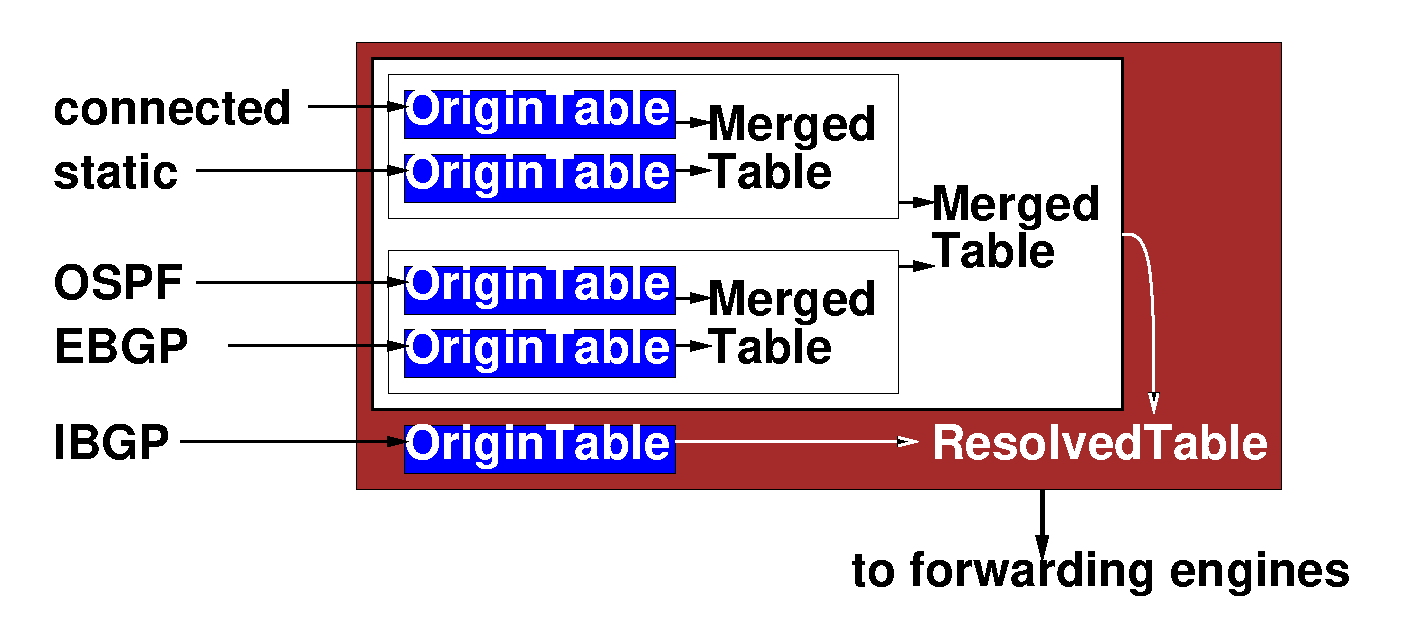
\epsfig{file=routingtable.ps,width=.8\hsize}
\end{center}
\B Object-oriented routing table design
\BB Add new merged tables implementing new merging policies, \dots
\end{slide}


\begin{slide}
\enlargethispage{4\baselineskip}
\T{Extensibility/performance: Click forwarding path}

\centering
\BTWO{4in}{4in}
\B Fast kernel forwarding
\B Easy to write extensions
\B XORP also supports native FreeBSD forwarding
\XTWO
\begin{center}
\epsfig{file=samp04_iprouter.1,scale=.6}
\end{center}
\ETWO

\end{slide}


\begin{slide}
\T{Robustness}

\B Policy decision: Strong robustness for user-level processes
\BB Difficult to get performance, robustness, and extensibility
simultaneously
\BB Kernel robustness through inspection of extensions
\B Facilitated by multi-process design
\BB Automatically restart processes that crash
\BB Defensive programming for shared XORP processes like RIB
\B XRL sandboxes
\BB All interaction with router through XRLs, packets
\BB Redirect XRLs to run new protocols in a sandbox
\end{slide}


\begin{slide}
\T{Status}

\B Core design, IPC, RIB, Click complete
\BB Routing tables, multicast, IPv6, Click integration in progress
\B All-new BGP, PIM-SM, IGMP in progress
\B Adapted OSPF, RIP in progress
\B First preliminary release within a month
\BB Check it out! Please help!
\end{slide}


\begin{slide}
\begin{center}
\Huge{\usefont{OT1}{DavidaBT}{b}{n}www.xorp.org}
\end{center}
\end{slide}


\end{document}
